\documentclass[10pt]{article}
\usepackage{blindtext}
\usepackage{amsfonts}
\usepackage{graphicx}
\usepackage{array}
\setlength{\parindent}{0em}
\newcolumntype{P}[1]{>{\centering\arraybackslash}p{#1}}
\graphicspath{ {/Users/Xiaopei/Documents/Coursework/Fall\ 2017/STATS\ M231/Project\ 3/Report}}
\usepackage[margin=1in]{geometry}
\title{Project 3: Fast R-CNN for Object Detection}
\author{Xiaopei Zhang (004309991)}
\date{\today}
\begin{document}
\maketitle
\section*{\large{Task 1: Single-class object detection in one image}}
	We use pre-trained Fast R-CNN model to do object detection in one example image. Figure 1 shows the number of detections over the value of threshold. The total number of bounding boxes after non-maximum suppression with a threshold of $0.15$ is $247$. We observe that as the threshold increases, the number of positive detections decreases, and we finalize the threshold as about $0.65$. 
	\\\\Figure 2 displays the car detections on the sample image.\\ 
	\begin{figure}[ht]
		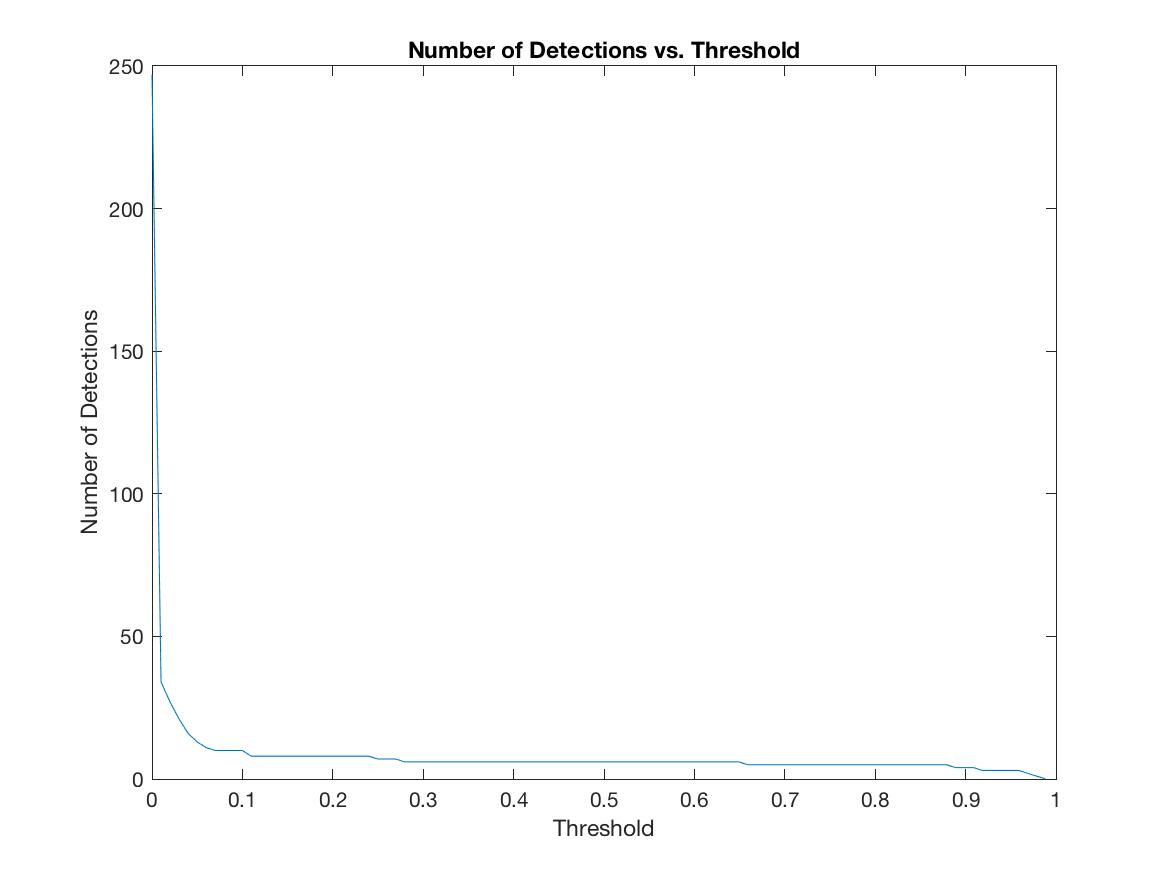
\includegraphics[width=\textwidth]{threshold_vs_numberOfDetection.jpg}
		\centering
		\caption{Number of detections over threshold.}
		\label{1}
	\end{figure}\\
	\begin{figure}[ht]
		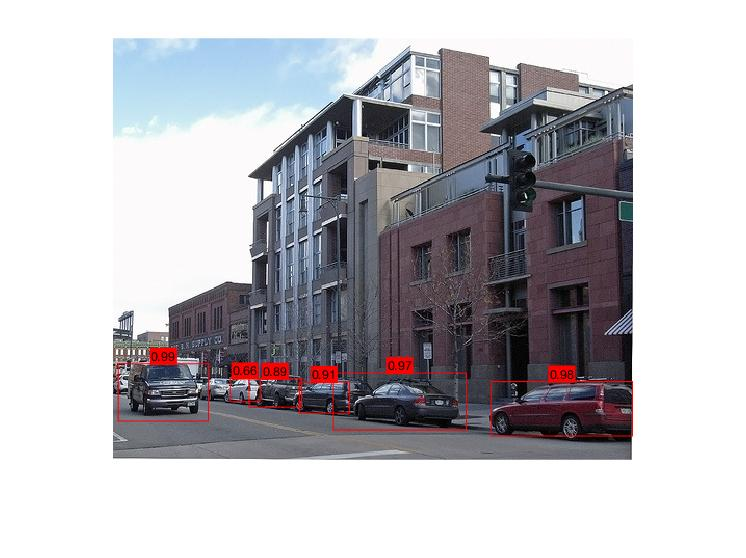
\includegraphics[width=\textwidth]{car_detection.jpg}
		\centering
		\caption{Car detections on the sample image.}
		\label{2}
	\end{figure}\\
\newpage\section*{\large{Task 2: Object detection on Pascal VOC 2007 dataset}}
	We use the same model to do object detection on testing dataset of Pascal VOC 2007. Figure 3 displays an example with true positive detections of multi-classes. In this example, the chairs, the potted plant, the dining table and the sofa can be considered as true positives, while the car and the person are false positives.\\
	\begin{figure}[ht]
		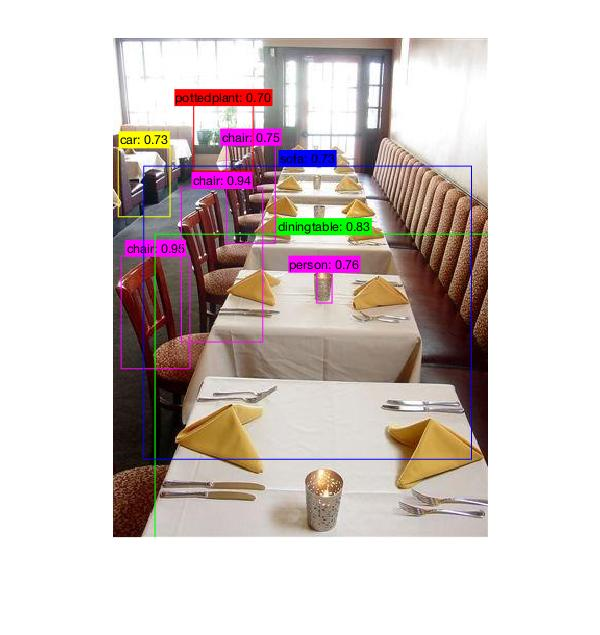
\includegraphics[scale = 0.75]{best_detection.jpg}
		\centering
		\caption{An example with true positive detections of multi-classes.}
		\label{3}
	\end{figure}\\
	\newpage To quantitatively the decision results, we plot the precision-recall curve for car class in Figure 4. From the curve, we observe that it is impossible achieve very high precision rate and recall rate simultaneously.\\
	\begin{figure}[ht]
		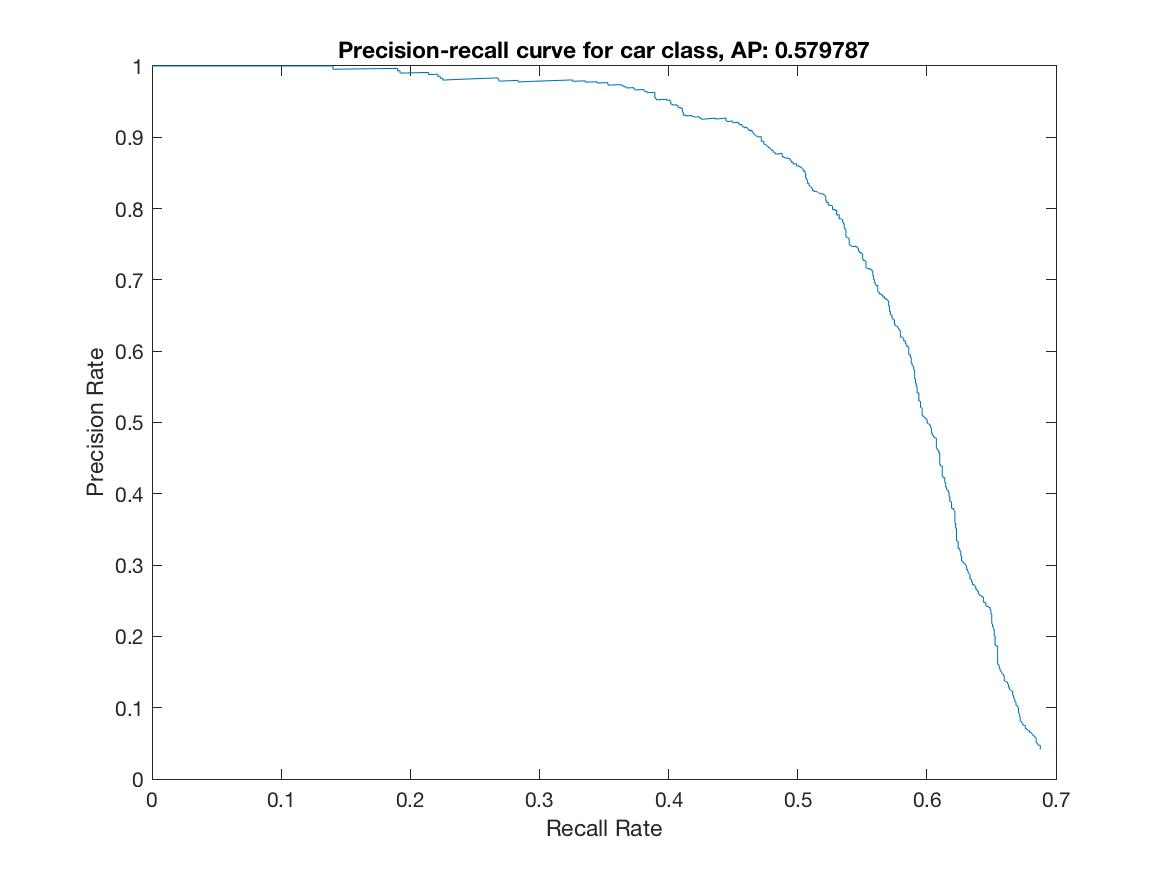
\includegraphics[width=\textwidth]{pr_curve_car.jpg}
		\centering
		\caption{Precision-recall curve for car class.}
		\label{4}
	\end{figure}\\
	\newpage Finally, we compute the average precision (AP) of every category and calculate the mean average precision (mAP) over 20 classes. Table 1 summarizes the results. From the table, we see that the mAP of our model is $0.481034$, which is good enough in general object detection.\\
	\begin{table}[ht]
 		\centering
 		\begin{tabular}{|c|c|}
		\hline
		Class & AP \\ \hline
		aeroplane & 0.585358  \\ \hline
		bicycle & 0.604260 \\ \hline
		bird & 0.406702  \\ \hline
		boat & 0.296687 \\ \hline
		bottle & 0.145479  \\ \hline
		bus & 0.615982 \\ \hline
		car & 0.579787  \\ \hline
		cat & 0.671733 \\ \hline
		chair & 0.206817 \\ \hline
		cow & 0.496006 \\ \hline
		dining table & 0.492875  \\ \hline
		dog & 0.567848 \\ \hline
		horse & 0.645948  \\ \hline
		motorbike & 0.610507 \\ \hline
		person & 0.477116  \\ \hline
		potted plant& 0.201672 \\ \hline
		sheep & 0.415092  \\ \hline
		sofa & 0.431161 \\ \hline
		train & 0.649127  \\ \hline
		tv monitor & 0.520533 \\ \hline
		total & 0.481034 \\ \hline
 		\end{tabular}
		\caption{Summary of average precisions for Pascal VOC 2007.}\label{tab1}
	\end{table}\\
\end{document}


Class: aeroplane, AP: 0.585358
Class: bicycle, AP: 0.604260
Class: bird, AP: 0.406702
Class: boat, AP: 0.296687
Class: bottle, AP: 0.145479
Class: bus, AP: 0.615982
Class: car, AP: 0.579787
Class: cat, AP: 0.671733
Class: chair, AP: 0.206817
Class: cow, AP: 0.496006
Class: diningtable, AP: 0.492875
Class: dog, AP: 0.567848
Class: horse, AP: 0.645948
Class: motorbike, AP: 0.610507
Class: person, AP: 0.477116
Class: pottedplant, AP: 0.201672
Class: sheep, AP: 0.415092
Class: sofa, AP: 0.431161
Class: train, AP: 0.649127
Class: tvmonitor, AP: 0.520533
mAP: 0.481034